\chapter{The Camera Module}

Cameras capture images.  Without them, the field of computer vision would not exist.  Whereas basic image processing algorithms operate on the 2-dimensional space of image pixels, most {\em computer vision} algorithms are distinguished by the fact that they will at some point tie the processed pixel data to objects in the real world for the purposed of measurement, tracking, or display.  This can only be done by modeling the geometric and physical properties of the device that was used to capture the original image.  This is the purpose of the camera module.

This module includes several built-in camera models for pinhole and line-scan imagers and a set of generic functions for linearizing (removing lens distortion) and epipolar rectifying (e.g. for stereo) camera models where these operations are relevant.  The user can provide their own camera model by inheriting from the {\tt CameraModel} abstract base class. Finally, the camera module provides a basic set of tools for working with images from real-world camera systems: bayer pattern filtering and EXIF parsing.  We will cover all of these in detail, however we begin this chapter by establishing some terminology while exploring one of the most ubiquitous camera models around: the pinhole camera model. 

\section{The Pinhole Camera Model}
The pinhole camera model is perhaps the most familiar to us, and we will use it here to help us establish some terminology that will be used throughout the rest of this chapter.  Please note that this model is somewhat simplistic; many of the non-ideal characteristics of a real-world optical system (e.g. lens distortion) are not modeled in this simple example, but should be modeled in the general case.  We will talk more about this in the sections below.

\subsection{Perspective Projection}

If the coordinates of ${\bf P}$ are $(x,y,z)$, then the position of the point on the imager can be determined by projecting it onto the plane $ z = +f$:

$$u = \frac{f}{\sigma} \left(\frac{x}{z}\right) + p_u$$
$$v = \frac{f}{\sigma} \left(\frac{y}{z}\right) + p_v$$

Here, $f$ is the focal length of the imager in meters, $\sigma$ is the size of a pixel in {\em m/pixel}, and $(p_u, p_v)$ are the offset in pixels of the principal point (this offset moves the origin of the image from the principal point to the lower left hand corner, from which images are generally indexed).

\begin{figure}[tbp]
\begin{center}
  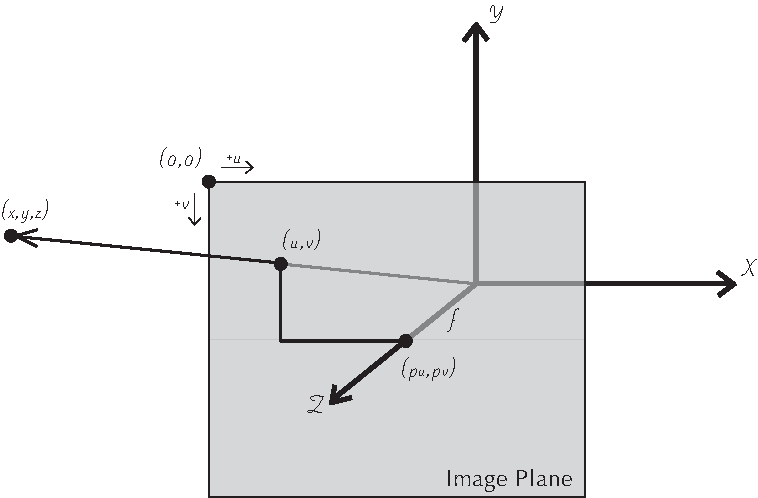
\includegraphics[width=5in]{images/camera_module_pinhole.pdf}
 \end{center}
  \label{fig:camera_module_pinhole}
  \caption{The basic pinhole camera model.}
\end{figure}
